\documentclass[tikz,border=6pt]{standalone}

\usepackage{amsmath}
\usetikzlibrary{arrows.meta}

\begin{document}

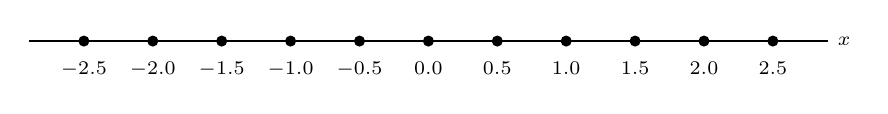
\begin{tikzpicture}[
  x=1.75cm,
  y=0.5cm,
  >=Stealth,
  font=\scriptsize
]

% Trục ngang biểu diễn x
% \draw[<->, line width=0.8pt] (-2.9,0) -- (2.9,0);
\draw[line width=0.8pt] (-2.9,0) -- (2.9,0);
\node[right] at (2.9,0) {$x$};

% Các điểm chia trên trục x
\foreach \xx in {-2.5, -2.0, -1.5, -1.0, -0.5, 0.0, 0.5, 1.0,1.5, 2.0, 2.5}{
  \fill (\xx,0) circle (2pt);
}

% Với y âm thì nhãn x đặt phía trên
\foreach \xx/\lab in {
  -2.5/{-2.5},
  -2.0/{-2.0},
   0.5/{0.5},
   1.0/{1.0},
   1.5/{1.5}
}{
  \node[below=4pt] at (\xx,0) {$\lab$};
}

% Với y dương (và y=0) thì nhãn x đặt phía dưới
\foreach \xx/\lab in {
  -1.5/{-1.5},
  -1.0/{-1.0},
  -0.5/{-0.5},
   0.0/{0.0},
   2.0/{2.0},
   2.5/{2.5}
}{
  \node[below=4pt] at (\xx,0) {$\lab$};
}

\end{tikzpicture}

\end{document}